\section{Introduction: information flow in Q-learning \label{Chapter7:Q learning application}}

This Section applies the information flow to an artificial agent
which uses reinforcement learning for an an obstacle avoidance task.
The purpose of the experiment is to prove that the same principles introduced
in the previous chapters apply to such a different on-line learning principle.
I will introduce first reinforcement learning, then describe the
robot-environment task with the learning controller and finally shows the
result of the application of the information flow.

\subsection{Methods: reinforcement learning }

Reinforcement learning \citep{TD} is characterised by a learning problem: an agent
learns from its interactions with the environment to achieve a goal.
Any method that is suited to solve this problem, is considered to be
a reinforcement learning method.
A reinforcement learning system is composed by:
\begin{itemize}
 \item the agent: the learner and decision maker decides to make an action $a_t$
 \item the environment: what interacts with the agent. It is described by a
state $s_t$ and gives a reward $r_{t+1}$ for each action.
 \item a policy $\pi_t$: a mapping from perceived states of the environment to
actions to be taken when in those states
 \item a reward function: a mapping from perceived states (or state-action pairs)
of the environment to a reward (a number).
The reward defines what are the good and bad events for the agent.
 \item a value function $V^{\pi}$: a mapping from perceived states to a value
which represents the expected total amount of reward that can be accumulated
over the future.
 \item optionally a model of the environment
\end{itemize}

The agent and the environment interact in time steps $t=0,1,2,3,4$
\footnote{for simplicity we assume a digital simulation but it can be extended
to the continuous case see \citep{TDrealtime}}.
At each time step t, the agent produces a representation of the environment's state,
$s_t \in S$, where  $S$
is the set of possible states and on that basis it takes an action $a_t \in A(s_t)$,
where $A(s_t)$ is the set of available actions in the state $s_t$.
One step later, the agent receives a numerical reward $r_{t+1}\in R$ and
find itself in a new state $s_{t+1}$.
At each time step the agent implements a mapping from states to probabilities
of selecting each possible action. The probabilities are
computed thanks to the agent's policy, where $\pi_t(s,a)$ is a mapping from
each state $s$ and action $a$ to the probability
of taking action  $a_t=a$ when in state $s_t=s$.
The vast majorities of reinforcement learning algorithms are based on estimating
the value function that estimates
how good it is for the agent to be in a given state. The positivity is defined in
terms of future rewards.
Thus, the value function $V^{\pi}(s)$, is the expected return when starting in
$s$ and following $\pi$ thereafter:
\begin{equation}
 V^\pi(s)=E{R_t|s_t=s}
\end{equation}
$V^{\pi}(s)$ is the state-value function for policy $\pi$.
There is also the complementary function $Q^\pi$ called the action-value function
for policy $\pi$: $Q^\pi$ is the the expected
 return starting from s, taking the action a, and thereafter following policy $\pi$:
\begin{equation}
 Q^\pi=E_\pi{R_t|s_t=s,a_t=a}
\end{equation}
Reinforcement learning methods specify how the agent changes its policy
as a result of its experience.
This framework is quite flexible and can be applied to different scenarios:
the states can be low-level sensations or they can be more
 abstracts like symbolic descriptions, the actions can be low level motor
commands or high level decisions like mental choices.
The general rule to define the boundary between the agent and the environment
is that anything that cannot be changed arbitrarily
by the agent is considered to be the environment.
The agent-environment boundary represents the limit of the agent's absolute control,
not of its knowledge. Indeed the agent may know
everything about its environment but the reward computation is out of the control
of the agent because it cannot be influenced arbitrarily.
The agent goal is to maximise the total amount of reward it receives in
the long run, in the simplest case of an
episodic task it is defined as:
\begin{equation}
 R_t=r_{t+1}+r_{t+2}+r_{t+3}+\cdots +r_T \label{eq:Qlearn.Rsimple}
\end{equation}
where T is a final time step. An episodic task, like playing a chess game
or solving a maze, is characterised by a terminal state, when
the agent ends up in this state, the environment is reset to its starting state.
If the goal requires a continuous-control, the final time T would be infinite and
therefore we cannot maximise an infinite time series,
therefore equation \ref{eq:Qlearn.Rsimple} needs to be modified as:

\begin{equation}
 R_t=r_{t+1}+\gamma r_{t+2}+ \gamma^2 r_{t+3}+\cdots =\sum_{k=0}^{\infty} \gamma^k r_{t+k+1} \label{eq:Qlearn.Rinf}
\end{equation}
where the parameter $\gamma$, $0\leq \gamma \leq 1$ is called the discount rate.
It determines the present value of future reward:
\begin{itemize}
 \item if $\gamma=0$, the agent maximises only immediate rewards and so
it chooses $a_t$ to maximise only $r_{t+1}$
 \item as $\gamma $ approaches 1, the agent consider future rewards more important.
\end{itemize}
The value functions $V^\pi$ and $Q^\pi$ are estimated from experience.
For example, if an agent follows the policy $\pi$
and maintains an average, for each state encountered, of the actual returns that
have followed that state, then the average
 will converge to the state's value, $V^\pi(s)$, as the number of times that
state is encountered approaches infinity.
If separate averages are kept for each action taken in that states, it will
converge to the action values, $Q^\pi(s,a)$.
The next section describes the connectionist Q-learning approach that will be
used by the agent for an obstacle avoidance task.

\subsection{Methods: Q-Learning algorithm}
The Q-Learning algorithm suggested by Watkins in 1989 [1] is one of the most popular
reinforcement learning algorithms.
In Q-Learning the purpose of the agent is to find a control policy $\pi$ which maximises the value function defined as:
\begin{equation}
 V(s_t) \leftarrow E{\sum_{k=0}^{\infty} \gamma ^k \cdot r_{t+k}}
\end{equation}
$V(s_t)$ depends on the sequence of actions determined by the policy $\pi$.
Q-Learning works on a Q-function which is computed from the value function in such a way:
\begin{equation}
Q(s_t,a_t) \leftarrow r_t +\gamma \cdot V(s_{t+1})
\end{equation}
where $a_t$ is an action chosen at time t out of the set of possible actions $A$.
Because the purpose of the system is to maximise the sum of total reward, $V(s_{t+1})$ is replaced by
$max_{a \in A} Q(s_{t+1},a)$ and thus the previous equation becomes:
\begin{equation}
Q(s_t,a_t) \leftarrow r_t +\gamma \cdot max_{a \in A} Q(s_{t+1},a)
\end{equation}
$Q$ is a 2-D table where the rows contains actions and the columns contains
states or vice-versa.
When the state-action space is large (especially in continuous cases) more
resources are required to store the table of evaluation.
To solve those problems, the following approaches were introduced in the literature:
\begin{itemize}
\item discretisation of the Q table: Q table of large size is split into several
Q tables of smaller size \citep{BartoSutton1983:Qtable}
\item Hamming distance approach
\item CMAC \nomenclature{CMAC}{Cerebellar Model Articulator Controller} method by Albus
\item RBF \nomenclature{RBF}{Radial Basis Functions} similar to CMAC
\item Neural Networks as suggested by Lin \citep{Lin92:memoryapproaches}
\end{itemize}
The following section describes the use of a a multilayer perceptron 
\nomenclature{MLP}{Multi Layer Perceptron Network} as a Q-
learning table approximation. The joint use of MLP
and the Q-learning algorithm is called connectionist Q-learning method.
\subsection{Methods: Q-Learning connectionist}
The tabular representation of the Q-function is replaced by a set of neural networks, each for every action.
States are forwarded to the inputs of the neural network and outputs are the estimates of the Q-values.
During each iteration of the learning algorithm, the current state of the system is forwarded to the inputs of
each neural network, but the weights are only updated for the network whose action was selected.
The weight correction error for the single step Q-learning is:
\begin{equation}
e_t=r_t+\gamma \cdot \max_{a \in A} Q(x_{t+1},a_{t+1})-Q(x_t,a_t)
\end{equation}
The modified connectionist Q-Learning algorithm is summarised with the following pseudo code:
\begin{enumerate}
 \item Set eligibility traces equal to zero, $e_0=0$
 \item Initialize time at $t=0$.
 \item Select an action, $a_t$
 \item If $t>0$, update the weights
 \item $w_t=w_{t-1} + \alpha \cdot ([r_{t-1}+\gamma \cdot \underset{a \in A}{\max Q_{t}} - Q_{t-1}]\cdot \triangledown_w Q_{t-1}
	    + [r_{t-1}+\gamma \cdot \underset{a \in A}{\max Q_{t}} - \underset{a \in A}{\max Q_{t-1}}]\cdot e_{t-1})$
 \item $e_t=\triangledown_w Q_{t} + \gamma \lambda e_{t-1}$ \\
       Calculate the output gradient $\triangledown_w Q_{t}$ only for the network whose action
	was chosen
 \item Execute action $a_t$ and receive reward $r_t$
 \item If the absorbing state is reached, then stop; otherwise $t \leftarrow t+1$ update time
and go to Step 3.
\end{enumerate}



\subsection{Methods: the robot and the task}
The robot is a Braitenberg vehicle as already described in Section \ref{WorldModelSim}
that can only execute 3 actions: move forward, turn left and right by a predefined angle.
The robot is situated in a square arena where 20 obstacles are placed randomly for each
session.
The task of the robot is to minimise the number of collisions by learning appropriate
motor responses from its sensory information.
The sensory information is generated by an array of floor binary sensors numbered
from 1 to 9 (see Figure \ref{fig:qlearning:robot}) that detect the presence
or absence of an obstacle on the world (binary input information).
The robot receives a reward signal $r(t)$ at time $t$
The geometric simulation parameters are described in the Appendix \ref{Appendix:QLearnSimDetails}.
The parameters for the MLP Q-learning algorithm are:
\begin{itemize}
 \item the learning rate is $\alpha=0.8$
 \item the forgetting rate for the eligibility traces is $\gamma=0.8$
 \item the Q-learning factor $\lambda=0.2$
\end{itemize}
The robot must receive a reward signal from the environment to be able to discriminate
between good and bad actions.
The reward structure was assigned in this way by the author:
\begin{itemize}
 \item $r(t)=0.1$ if at time $t$ the robot has moved forward successfully
 \item $r(t)=-0.2$ if at time $t$ the robot has collided with an obstacle
 \item $r(t)=0$ if at time $t$ the robot has collided with a wall of the world
\end{itemize}

\begin{figure}[tbp]
\begin{center}
\includegraphics[width=0.6 \textwidth]{qlearning/Q-Learning-Robot.eps}
\end{center}
\small{
\caption[Q learning robot]{Simplified diagram of the q-learning robot.
The yellow dots represent a binary input for the detection of the obstacle.
 \label{fig:qlearning:robot}}}
\end{figure}

For each simulation (see Figure \ref{fig:qlearning:robot-sim1}) the robot goes
through three different stages:
\begin{itemize}
 \item in $T_0=[0,1\cdot 10^6]$ the robot is purely reactive and does not learn by
imposing $\lambda=0.0$
 \item in $t=(1\cdot  10^6, 2 \cdot  10^6]$ the robot fully learning by
imposing $\lambda=0.8$
 \item in $T_\infty=(2 \cdot  10^6, 4 \cdot  10^6]$ the robot has learned from the previous
section and now uses his weights $w$ to avoid the obstacles.
\end{itemize}

\begin{figure}[tbp]
\begin{center}
\includegraphics[width=0.8 \textwidth]{qlearning/robotreflexsim1.eps}
\end{center}
\small{
\caption[Q learning environment]{The obstacles are marked as yellow at the beginning.
When an obstacle is touched it becomes orange to keep track of the collision history.
The number of collisions and the average reward are shown in the simulation window.
The red status label describes in what stage the robot is.
 \label{fig:qlearning:robot-sim1}}}
\end{figure}

\subsection{Results: avoidance case}
The information flow is calculated as in the previous Section \ref{Chapter6:Information Flow},
but in this case it is very easy because the output $Z$ and the input $S$ of the robot
are already discrete.
The input $S$ is a binary word of 9 bits:
\begin{equation}
S={S_1 S_2 S_3 S_4 S_5 S_6 S_7 S_8 S_9}  \label{eq:qlearn:S}
\end{equation}
where each bit indicates if the sensor has touched the obstacle.
For example the string $S={1 0 0 1 0 0 0 0 0}$ indicates that the obstacle has
collided with the input sensor in position 1 and 4 (see Figure \ref{fig:qlearning:robot}).
The output $Z$ is encoded with a word of 2 bits:
\begin{equation}
Z={Z_1 Z_2}   \label{eq:qlearn:Z}
\end{equation}
which encodes the 3 possible actions:
\begin{itemize}
 \item move forward $Z_{fwd}={0 0}$
 \item turn left    $Z_{left}={0 1}$
 \item turn right   $Z_{right}={1 0}$
\end{itemize}
in this case 1 combination $Z_{null}={0 0}$ is not used because there are
only 3 actions performed by the robot.
To apply the information measure described in the Section \ref{Chapter6:Information Flow},
it is necessary to distinguish between the proximal or reflex signal X and the
distal signal Y.
The sensor inputs numbered 1,4,7 are far from the robot and thus can be
regarded as distal inputs, whereas the inputs 3,6,9 are closer to the robot
and thus can be regarded as proximal or reflex signals.
\begin{itemize}
 \item $MI(X,Z)$ is the mutual information between the output Z and the reflex input X
 \item $MI(Y,Z)$ is the mutual information between the output Z and the distal input Y
\end{itemize}
$X$ is thus encoded with a 3 bit word, $Y$ is encoded as a 3 bit word and
$Z$ as described before as a 2 bit word.
The information flow is computed from the previous quantities, by concatenating
the output Z $n$ times:
\begin{itemize}
 \item $MI^n(X,Z)$ is the information flow of order n between the output Z and the reflex input X
 \item $MI^n(Y,Z)$ is the information flow of order n between the output Z and the distal input Y
\end{itemize}
I then calculated the reflex and distal information flow for the robot during the purely reflex phase and after learning.
Table \ref{tab:Qlearning:infoflowtable-worandom} shows the relevant values
for a typical simulation run before and after learning:
\begin{itemize}
 \item because the agent has an instantaneous motor response, the order was computed
for $n=4,5,6$ actions
\item $R_0$ indicates the average reward received by the robot before learning
\item $R_\infty$ indicates the average reward received by the robot after learning
\end{itemize}
Table \ref{tab:Qlearning:infoflowtable-wrandom} shows the same results for the
same robot but with a 10\% probability of choosing random actions during learning.
This strategy increases the exploration probability and results in a better
performance because $R_\infty=0.0791>0.0688$ for the case without random selection.
The clear result is that when the robot is learning is reducing the reflex information
flow $MI(X,Z)$ and increasing the predictive information flow $MI(Y,Z)$,
even though this behaviour was not designed but learned by the Q-learning approach.
For example, if I consider the information flow of order 5 from Table \ref{tab:Qlearning:infoflowtable-wrandom},
before learning the robot is using $MI^{5}(X,Z)=1.0446$ bits in the reflex loop
and only $MI^{5}(Y,Z)=0.0376 $ bits in the predictive loop but after learning,
the robot is using less information from the reflex loop $MI^{5}(X,Z)=0.0271$ and
more information from the predictive loop $MI^{5}(Y,Z)=1.8086 $ bits.
Same interpretation applies to the other cases described in the tables.

\begin{table}[htbp]
\addtolength{\tabcolsep}{-2pt}
\centering
\begin{tabular}{| c|| c| c | c| c | c | c |}
\hline
$\underbrace{Order}_ n$& $\underbrace{MI(X,Z)}_{T_0}$& $\underbrace{MI(Y,Z)}_{T_0}$ & $R_0$ & $\underbrace{MI(X,Z)}_{T_\infty}$& $\underbrace{MI(Y,Z)}_{T_\infty}$ & $R_\infty$ \\
\hline
4 & 0.0965 & 0.0864 & 0.0429 & 0.0102 & 0.3691 & 0.0688 \\
\hline
5 & 1.0815 & 0.0864 & 0.0429 & 0.103 & 0.3747 & 0.0688 \\
\hline
6 & 0.0965 & 0.0874 & 0.0429 & 0.0104 & 0.3824 & 0.0688 \\
\hline
\end{tabular}
\caption[Information flow for avoidance robot]{Table containing the information flow when
the robot is avoiding the obstacles without random selection of the actions. \label{tab:Qlearning:infoflowtable-worandom}}

\end{table}

\begin{table}[htbp]
\addtolength{\tabcolsep}{-2pt}
\centering
\begin{tabular}{| c|| c | c | c | c| c | c |}
\hline
$\underbrace{Order}_ n$& $\underbrace{MI(X,Z)}_{T_0}$& $\underbrace{MI(Y,Z)}_{T_0}$ & $R_0$ & $\underbrace{MI(X,Z)}_{T_\infty}$& $\underbrace{MI(Y,Z)}_{T_\infty}$ & $R_\infty$ \\
\hline
4 & 0.0521 & 0.0481 & 0.0473 & 0.0249 & 0.7861 & 0.0791 \\
\hline
5 & 1.0446 & 0.0376 & 0.0473 & 0.0271 & 1.8086 & 0.0791 \\
\hline
6 & 0.0523 & 0.0484 & 0.0473 & 0.0303 & 0.8240 & 0.0791 \\
\hline
\end{tabular}
\caption[Information flow for avoidance robot]{Table containing the information flow when
the robot is avoiding the obstacles with random selection of the actions at 10\%. \label{tab:Qlearning:infoflowtable-wrandom}}

\end{table}

\subsection{Discussion}
The application of the information flow to this simple case of obstacle avoidance,
gives an insight about the actual learning outcome of the robot.
Before learning the robot uses a mixed combination of close and far sensors,
whereas after learning the robot decreases the use of the close sensors
for the benefit of the far ones.
The initial use of the information flow is different for the ICO learning case
which is programmed to use the reflex stimuli as a sort of wired behaviour.
The Q-learning does not have any hard wired behaviour but only a random
initialisation of the weights in the neural network and thus there is no preference
between the stimuli.
After learning the algorithm it discovers that is not a good idea to react
when the obstacle is too close even though the rewards are identical for
a close or far collision.
Although the computation of the information flow shows a clear development of 
behaviour from reactive to predictive, in ICO the reflex acts as the ``reward'' or 
the punishment channel in relation to Q-learning.
Thus a more intuitive approach would have been to compute the two mutual 
informations $MI(R,Z)$ between output and reward as the reflex loop and $MI(Y,Z)$
between output and distal input.
The main disadvantage of using this approach is that due to the sparsity of the 
reward signal it is necessary to use a more complex information model and was avoided
to have a more behavioural based measure where we know how the agent is using
its input differently.
In summary by comparing the ICO approach with the Q-learning approach,
there is similarity in terms of the strategy adopted by the robot in this particular
scenario.
It would be interesting to investigate if the similar property holds for
different experimental setups where the task is not just attraction or avoidance.
This investigation was not carried further in the Thesis as it was far away from the
main topic but it is certainly something that can be investigated in the future.

